% Chapter 3

\chapter{Geles polim\'ericos} % Main chapter title

\label{Chapter3} % For referencing the chapter elsewhere, use \ref{Chapter1} 

%----------------------------------------------------------------------------------------

% Define some commands to keep the formatting separated from the content 
\newcommand{\keyword}[1]{\textbf{#1}}
\newcommand{\tabhead}[1]{\textbf{#1}}
\newcommand{\code}[1]{\texttt{#1}}
\newcommand{\file}[1]{\texttt{\bfseries#1}}
\newcommand{\option}[1]{\texttt{\itshape#1}}

%----------------------------------------------------------------------------------------

\section{Modelo sencillo: 2 fases}

Microgels are soft particles made of crosslinked polymer chains that can display both colloidal and macromolecular behavior \addcite[plamper2017,lyon2012].
Immersed in aqueous solutions, these particles incorporate and retain large amounts of water within their polymeric structure.
Typically, their diameters range from tens of nanometers (nanogels) up to several microns.
However, the most striking feature of these particles is their ability to uptake or release solvent and change size in response to a variety of external stimuli.
Such responsive behavior is reversible and depends on the chemical composition of the polymer network.


Microgels composed of polymer chains having acidic segments such acrylic or methacrylic acid (AA and MAA, respectively) swell/deswell many-times fold in response to changes in the solution pH \addcite[snowden1996,Zhou1998].
The particular pH that marks the onset and characterizes this transition is the apparent pKa of the microgel, which depends on the solution salt concentration and frequently differ from the intrinsic pKa of the acidic monomer.
These microgels also adjust their size in response to changes in the salt concentration of the solution \addcite[snowden1996].




Analogously, microgels of some thermoresponsive polymers undergo a volume phase transition (VPT) when heated above a characteristic temperature (VPTT or Tpt)\addcite[Pelton1986,Pelton2000].
This behavior originates because such polymers are insoluble in water above a certain lower critical solution temperature (LCST) \addcite[Kawaguch2020].
Typically, the LCST of the polymer and the VPTT of the crosslinked network are roughly identical.
This is the case for microgel particles of crosslinked poly(N-isopropylacrylamide) (PNIPAm) \addcite[Pelton1986], whose volume collapse above $32 C$, the LCST of the linear polymer \addcite[Schild1992].

Having a VPTT around body temperature, PNIPAm microgels have generated great interest for biomedical applications \addcite[Guan2011].
Strategies for controlling the VPTT of microgels include the synthesis of novel thermoresponsive monomers\addcite[Cai2007,Macchion2019] as well as copolymerization of with an ionic or ionizable monomer \addcite[Hirose1987, Lopez2010].
This latter approach yields multiresponsive microgels that are susceptible to changes in temperature, pH and salt concentration \addcite[snowden1996, Farooqi2017].
Microgels of N-isopropylacrylamide (NIPAm) and AA have been widely studied \addcite[Morris1997, Jones2000, Bradley2005, Begum2016]; 
microgels of NIPAm and MAA copolymers have also been investigated \addcite[Dowding2000, Hoare2004, Giussi2015].
The VPTT of these multiresponsive microgels depends on the solution pH and salt concentration, and the fraction of ionizable monomer in the polymer chains \addcite[Morris1997, Jones2000, Hoare2004, Bradley2005, Lee2008, Wong2009, Hamzavi2016].
In addition, the incorporation of the acidic comonomer provides a pH-controlled mechanism for the uptake/release of oppositely charged molecules, which makes multiresponsive microgels attractive for the design of functional drug delivery systems \addcite[Liu2017].



Applications based on polymer microgels are becoming more diverse and increasingly important in different areas of technology \addcite[plamper2017].
Nanocomposites made of poly(NIPAm-\emph{co}-MAA) microgels that incorporate gold or silver nanoparticles or metal organic frameworks have potential applications 
in the development of materials with tunable catalytic activity
for the degradation of industrial pollutants \addcite[Khan2013, Shi2014, Allegretto2020].
These microgels can also be applied for the development of pH, salt and temperature-responsive emulsions  \addcite[Ngai2005, Ngai2006, Brugger2008, Schmidt2011] or as templates for the assembly of nanomaterials \addcite[Wong2009].
Multiresponsive nano/micro-sized polymer gels are excellent candidates for the development of minimally invasive biomedical applications, including granular scaffolds for tissue engineering \addcite[Daly2020].
\addcite[citet:Culver2017A] have used functionalized poly(NIPAm-co-MAA) nanogels for the binding and sensing of different proteins.
Devices based on poly(NIPAm-co-MAA) microgels have been recently investigated for the encapsulation/release of the chemotherapeutic drug Doxorubicin \addcite[Giussi2020, MartinesMoro2020, Pergushov2020].

In this context, here we derive a two-phase equilibrium theory and perform a systematic investigation of the thermodynamic behavior of microgels composed of random copolymers of NIPAm and an acidic comonomer.
This model describes the physical chemistry behind all of the following phenomena: the pH-driven microgel swelling, the nonmonotonic dependence of particle size on the salt concentration, and the network collapse when increasing the temperature above the VPTT.
Our predictions provide a clear picture of the effects of solution composition (pH, salt concentration) and polymer chemistry (MAA content, degree of crosslinking) on the VPT.
We also investigate the best conditions for Doxorubicin and Daunorubicin encapsulation within these microgels.
Our calculations are specific to methacrylic acid with $pKa = 4.65$, but the physicochemical behavior reported can qualitatively describe a variety of NIPAm-based microgels that have been modified with other acidic monomers having different pka and different solubility at low pH.


The behavior of poly(NIPAm-co-MAA) microgels, including their VPT and interaction with oppositely charged polymers, has been described using a variety of experimental techniques \addcite[Hoare2004,Dowding2000, Kleinen2008, Kleinen2010, Giussi2015, Su2016, Giussi2020].
Theory and coarse grained molecular simulations have also been applied to investigate the behavior stimuli-responsive polymer microgels \addcite[quesada2011gel, ahualli2016coarse, Landsgesell2019SM].
These works have mainly focused on the swelling and other properties of particles having a permanently charged polymer network \addcite[Levin2002,Claudio2009,Colla2014,Jha2011,jha2012understanding,QuesadaPerez2013,QuesadaPerez2014,Kobayashi2014,Kobayashi2016,Rizzi2016,moncho-jorda2016a,Kobayashi2017,AdroherBenitez2017PCCP], and some have addressed the effect of temperature and solvent quality \addcite[Jha2011,QuesadaPerez2013,QuesadaPerez2014,moncho-jorda2016a,ahualli2016coarse,AdroherBenitez2017PCCP]. 
Recently, simulation studies have considered the pH-response of microgels composed of charge-regulating polymers\addcite[Schroeder2015, Rudov2017, Sean2018, Hofzumahaus2018, Lu2019].
Only a few theoretical works, however, have investigated the properties of  multiresponsive microgels as a function of temperature, pH and salt concentration \addcite[CaprilesGonzalez2008, polotsky2013collapse].

\subsection{Microgel Phase}\label{sec:theory}
%%%%%%%%%%%%%%%%%%%%%%%%%%%%%%%%%%%%%%%%%%%%%%%%%%%%%%%%%%%%%%%%%%%%%


Let us consider a model of two phases: a poly(NIPAm-\emph{co}-MAA) (P(NIPAm-MAA)) microgel (phase $1$, denoted by $MG$) in contact with an embedding aqueous solution (phase $2$, denoted by $s$).
Externally, we can control the temperature $T$, the pH and salt concentration of this solution, which result in the microgel having radius $R$ and volume $V=\frac{4}{3}\pi R^3$.
The thermodynamic potential whose minimum yields the equilibrium conditions inside the microgel phase is the semi-grand canonical potential, $\Omega_{MG}$, which contains the following contributions:
%
\begin{align}
    \begin{aligned}
       \Omega_{MG}=& -TS_{mix} + F_{chem,MAA} +  F_{ela}\\
       & + U_{elec}+  U_{ste} + U_{VDW} -{\sum_{\gamma}
        {\mu_\gamma N_\gamma}}
    \end{aligned}
    \label{eq:free-energy-implicit}
\end{align}
%
\noindent where $S_{mix}$ is the translational (mixing) entropy of the free species in the microgel phase: water molecules ($w$), hydronium ($H_3O^+$) and hydroxyde  ions ($OH^-$), and salt cations ($+$) and anions ($-$). 
Here we consider a monovalent salt, $KCl$, and assume it is completely dissociated into potassium and chloride ions.
$F_{chem,MAA}$ is the chemical free energy that describes the equilibrium protonation of MAA units.
$F_{ela}$ is the elastic free energy that accounts for the conformational freedom of the polymer network.
$U_{elec}$ and $U_{ste}$ account respectively for the electrostatic interactions and steric repulsions.
$U_{VDW}$ is the contribution that describes the polymer-solvent effective interactions; it incorporates the hydrophilic-hydrophobic transition of NIPAm upon increasing the temperature above its LCST.
Finally, the sum over $\gamma$ expresses the chemical equilibrium with the solution phase, where $\mu_\gamma$ and $N_\gamma$ are the chemical potential and number of molecules of species $\gamma$, respectively.
Herein, the subindex $\gamma$ runs over the free chemical species, $\gamma \in \left\{ w, H_3O^+, OH^-, +,- \right\}$.
Note that $\Omega_{MG}$ is a semi-grand canonical potential because the microgel phase can exchange each of these molecules with the solution phase, while the polymer network is confined within the former.

The explicit form of the thermodynamic potential is: 
%
\begin{align}
\begin{aligned}
\beta&\frac{\Omega_{MG}(R)}{V}=\\& ~ \sum_{\gamma} \rho_\gamma\left(\ln\left(\rho_\gamma v_w\right) -1 + \beta\mu^0_\gamma\right) \\
& + \frac{\phi_{MAA}}{v_{MAA}} \left[f(\ln f+ \beta\mu^0_{MAA^-})\right.\\
&\qquad\left.+(1-f)(\ln (1-f)+\beta\mu^0_{MAAH})\right] \\
%
& +  \left(\sum_{\gamma } {\rho_\gamma q_\gamma + f\dfrac{\phi_{MAA}}{v_{MAA}}q_{MAA}}\right)\beta\psi_{MG}\\
%
& -\sum_{\gamma }{\rho_\gamma\beta\mu_\gamma}
 -\beta\mu_{H^+}(1-f)\dfrac{\phi_{MAA}}{v_{MAA}}\\
%
& + \chi (T, \phi_{NIPAm})\rho_w \phi_{NIPAm} \\
%
& + \dfrac{3}{2}\dfrac{N_{seg}}{n_{ch} V}\left[\left(\dfrac{R}{R_0}\right)^2 - \ln\dfrac{R}{R_0} -1\right]
%
\end{aligned}
\label{eq:free-energy}
\end{align}


\noindent where the first term (second line) arises from $S_{mix}$; $\beta=\frac{1}{k_BT}$ and $k_B$ is the Boltzmann constant.
The number density of species $\gamma$ is $\rho_\gamma$ and $\mu^0_\gamma$ is its  standard chemical potencial, which is also included in this first contribution; $v_w$ is the volume of a water molecule.



The second and third line of eq. \ref{eq:free-energy} (right-hand side) incorporate the acid-base equilibrium of MAA units, where $\phi_{MAA}$ is the volume fraction that these segments occupy, $v_{MAA}$ is the volume of this segment, and $f$ is the degree of dissociation or the fraction of these units that are charged.
The volume fraction of charged MAA segments is $f\phi_{MAA}$, and that of protonated or uncharged units is $(1-f)\phi_{MAA}$.
The standard chemical potentials are $\mu^0_{MAA^-}$ and $\mu^0_{MAAH}$ for the charged and protonated species, respectively.
Note that here we use the term segment to identify the chemical units (monomers) that compose the polymer chains (MAA and NIPAm).


The next contribution to eq. \ref{eq:free-energy} is the electrostatic energy, where $q_\gamma$ and  $q_{MAA}$ are the electric charge of molecules $\gamma$ and MAA segments, respectively. 
The electrostatic potential inside the microgel phase is $\psi_{MG}$.


The following contribution (line 6 of eq.\ref{eq:free-energy}) reinforces the chemical equilibrium between the microgel and the solution phase, where the second term accounts for those protons bound to uncharged MAA units; 
namely, $\mu_{H^+}\equiv\mu_{H_3O^+}$ is conjugated to the total number of protons,
$N_{H_3O^+}+N_{MAAH}=V\left(\rho_{H_3O^+}+(1-f)\dfrac{\phi_{MAA}}{v_{MAA}}\right)$.


The next term in the thermodynamic potential accounts for PNIPAm response to temperature changes through a polymer solvent interaction parameter, $\chi$, which depends on the temperature and the volume fraction of NIPAm, $\phi_{NIPAm}$.
According to \addcite[afroze2000], this Flory-Huggins parameter can be expressed as:
%
%
\begin{align}
\begin{aligned}
\chi (T, \phi_{NIPAm}) &=g_0(T) +g_1(T)\phi_{NIPAm} \\
 &~+ g_2(T)\phi_{NIPAm}^2
\end{aligned}
\end{align}

\noindent with
%
%
\begin{align}
\begin{aligned} 
g_k(T)=g_{k0} + \frac{g_{k1}}{T} + g_{k2}T
\end{aligned}
\end{align}


\noindent for $k=0,1,2$, where the coefficients are $g_{00}= -12.947$, $g_{02}=0.044959\,$K$^{-1}$, $g_{10}= 17.920$, $g_{12}= -0.056944$\,K$^{-1}$, $g_{20}= 14.814$, $g_{22}= -0.051419$\,K$^{-1}$ and $g_{k1}\equiv 0$ \addcite[afroze2000]. 


The last term in eq. \ref{eq:free-energy} is the contribution resulting from the elasticity of the crosslinked polymer network that makes the microgel backbone.
This expression is described in \addcite[mocho-jorda2016a] and comes from the model of rubber elasticity, 
where $N_{seg}$ is the total number of segments in the polymer network, and $n_{ch}$ is number of segments per polymer chain or \emph{chain length}.
Note that the spring constant in the elastic free energy is proportional to the quotient $\dfrac{N_{seg}}{n_{ch}}$, which represents the (total) number of polymer chains in the microgel.
The radius of the dry microgel is $R_0$, which satisfies:
%
%
\begin{align}
\begin{aligned} 
\dfrac{4}{3}\pi R_0^3=V_0&=N_{seg}\Big( x_{MAA} v_{MAA}\\
&\qquad+x_{NIPAm} v_{NIPAm}\Big)
\end{aligned}
\end{align}

\noindent where $V_0$ is the volume of the dry particle; $x_{MAA}$ and $x_{NIPAm}$ are the fraction of MAA and NIPAm segments, respectively.
Then, the total number MAA segments is $x_{MAA}N_{seg}$ and that of NIPAm units is $x_{NIPAm}N_{seg}$, each having a volume $v_{NIPAm}$.
The microgels we consider here satisfy $x_{NIPAm}=1-x_{MAA}$.


Two physical constraints must be imposed to the thermodynamic potential given by eq. \ref{eq:free-energy}.
The microgel volume is fully occupied by network segments and the free chemical species.
This incompressibility constraint incorporates the steric repulsions (excluded volume) and can be expressed as:
%
%
\begin{align}
\begin{aligned}
\sum_{\gamma } \rho_\gamma v_\gamma  + \phi_{MAA} + \phi_{NIPAm} = 1
\end{aligned}
\label{eq:packing}
\end{align}



\noindent where $v_\gamma$ is the molecular volume of specie $\gamma$, and
the volume fractions of network components are: 
%
%
\begin{align}
\phi_{MAA}&=N_{seg}\dfrac{x_{MAA}v_{MAA}}{\frac{4}{3}\pi R^3}\\
\phi_{NIPAm}&=N_{seg}\dfrac{x_{NIPAm}v_{NIPAm}}{\frac{4}{3}\pi R^3}
\end{align}



The second constraint that we impose to the microgel phase is charge neutrality, which can  be expressed as: 
%
%
\begin{align}
\begin{aligned}
\sum_{\gamma  } \rho_\gamma q_\gamma + f\frac{\phi_{MAA}}{v_{MAA}}q_{MAA}=0
\end{aligned}
\label{eq:charge-neutrality}
\end{align}


Now, the thermodynamic potential is an explicit function of the densities of all free species, the degree of charge of MAA segments and the radius of the microgel, $\Omega_{MG}(R)\equiv\Omega_{MG}(\{\rho_\gamma\},f,R)$.
To obtain the expressions of $\{\rho_\gamma\}$ and $f$ that are consistent with the thermodynamic equilibrium, we minimize $\Omega_{MG}$ with respect to these quantities, subject to the constraints eq. \ref{eq:packing} and eq. \ref{eq:charge-neutrality}; such procedure leads to
%
%
\begin{align}
\rho_\gamma v_w &= a_\gamma \exp(-\beta\pi_{MG}v_\gamma -\beta\psi_{MG}q_{\gamma})\\
\frac{f}{1-f}&= \frac{K^0_{MAA}}{a_{H^+}}\exp(-\beta\psi_{MG}q_{MAA})\label{eq:fcharge}
\end{align}


\noindent where $a_\gamma = e^{\beta\mu_\gamma-\beta\mu_\gamma^0}$ is the activity of species $\gamma$, and $\pi_{MG}$ is the osmotic pressure of the microgel phase, introduced as a Lagrange multiplier to impose the incompressibility constraint, eq. \ref{eq:packing}.
The thermodynamic equilibrium constant that describes MAA protonation/deprotonation is
%
%
\begin{align}
K^0_{MAA}= e^{\beta\mu^0_{MAAH}-\beta\mu^0_{MAA}-\beta\mu^0_{H^+}}
\end{align}

\noindent This quantity can be directly calculated from the pKa of the acid.




For a given $R$, the only remaining unknowns to determine $\Omega_{MG}(R)$ are the osmotic pressure, $\pi_{MG}$ and the electrostatic potential, $\psi_{MG}$.
These two quantities can be calculated through numerically solving the incompressibility and the electroneutrality of the microgel phase, eq. \ref{eq:packing} and eq. \ref{eq:charge-neutrality}, respectively. 
To solve these equations we use a Jacobian-free Powell hybrid method and a FORTRAN code developed in-house.


All other quantities involved in the calculation of $\Omega_{MG}(R)$ are inputs, including the properties of the different chemical species considered, which are summarized in table \ref{table:molecules}.
We use $pK_w=14$ to describe water self-dissociation equilibrium.
The activities of all free chemical species can be calculated from the concentration of these molecules in the solution phase as discussed next.


\begin{table}
	\centering
%\small
%\begin{tabular}{lcS[table-format=-1]S[table-format=0.3]}
\begin{tabular}{|lccc|}
    \hline
    {Species} & {$pKa$} & {$q$ ($e$)} & {$v$ ($\text{nm}^3$)} \\
      \hline
$H_2O\,(w)$ & ~ & ~ & 0.03\\
$H_3O^+$ & ~ & +1 & 0.03\\
$OH^-$ & ~ & -1 & 0.03\\
$K^+\,(+)$ & ~ & +1 & 0.04\\ 
$Cl^-\,(-)$ & ~ & -1 & 0.047\\
$MAA$ & 4.65 & -1$^\ast$ & 0.09\\
$NIPAm$ & ~ & ~ & 0.12\\
    \hline
  \end{tabular}
 \caption{Molecular properties of the different chemical species considered.
 \footnotesize ($^\ast$For the deprotonated species.)}
\label{table:molecules} 
\end{table}


%%%%%%%%%%%%%%%%%%%%%%%%%%%%%%%%%%%%%%%%%%%%%%%%%%%%%%%%%%%%%%%%%%%%%
\subsection{Solution Phase}
%%%%%%%%%%%%%%%%%%%%%%%%%%%%%%%%%%%%%%%%%%%%%%%%%%%%%%%%%%%%%%%%%%%%%

In the solution, the thermodynamic potential is:
%
%
\begin{align}
\begin{aligned}
\beta&\frac{\Omega_s}{V}=\\& \sum_{\gamma   } {\rho^s_\gamma\left(\ln(\rho_\gamma^sv_w) -1 + \beta\mu_\gamma^0 - \beta\mu_\gamma\right)}
\end{aligned}
\label{eq:bulk}
\end{align}

\noindent where the superscript $s$ indicate solution densities.
In writing eq. \ref{eq:bulk}, we have considered a reference volume equal to that of the microgel, $V$, and set the electrostatic potential in the solution phase equal to zero.




Once the solution composition is set (pH and salt concentration), we know the densities of all chemical species in this phase, which must satisfy both the incompressibility and charge neutrality constraints: 
%
%
\begin{align}
\sum_{\gamma  } \rho_\gamma^s v_\gamma  &=1\label{eq:bulk-packing}\\
\sum_{\gamma  } \rho_\gamma^s q_\gamma  &=0
\end{align}

\noindent with
%
%
\begin{align}
\rho_\gamma^s v_w= a_\gamma \exp(-\beta\pi_s v_\gamma)
\label{eq:bulk-electroneutrality}
\end{align}



\noindent for $\gamma \in \left\{ w, H_3O^+, OH^-, +,- \right\}$, where $\pi_s$ is the osmotic pressure of the solution phase introduced as a Lagrange multiplier to reinforced eq. \ref{eq:bulk-packing}.
After $\pi_s$ is known, we can determine the activities of all free chemical species.

\subsection{Graphical Minimization}
%%%%%%%%%%%%%%%%%%%%%%%%%%%%%%%%%%%%%%%%%%%%%%%%%%%%%%%%%%%%%%%%%%%%%

\begin{figure*}[!htb]
\centering
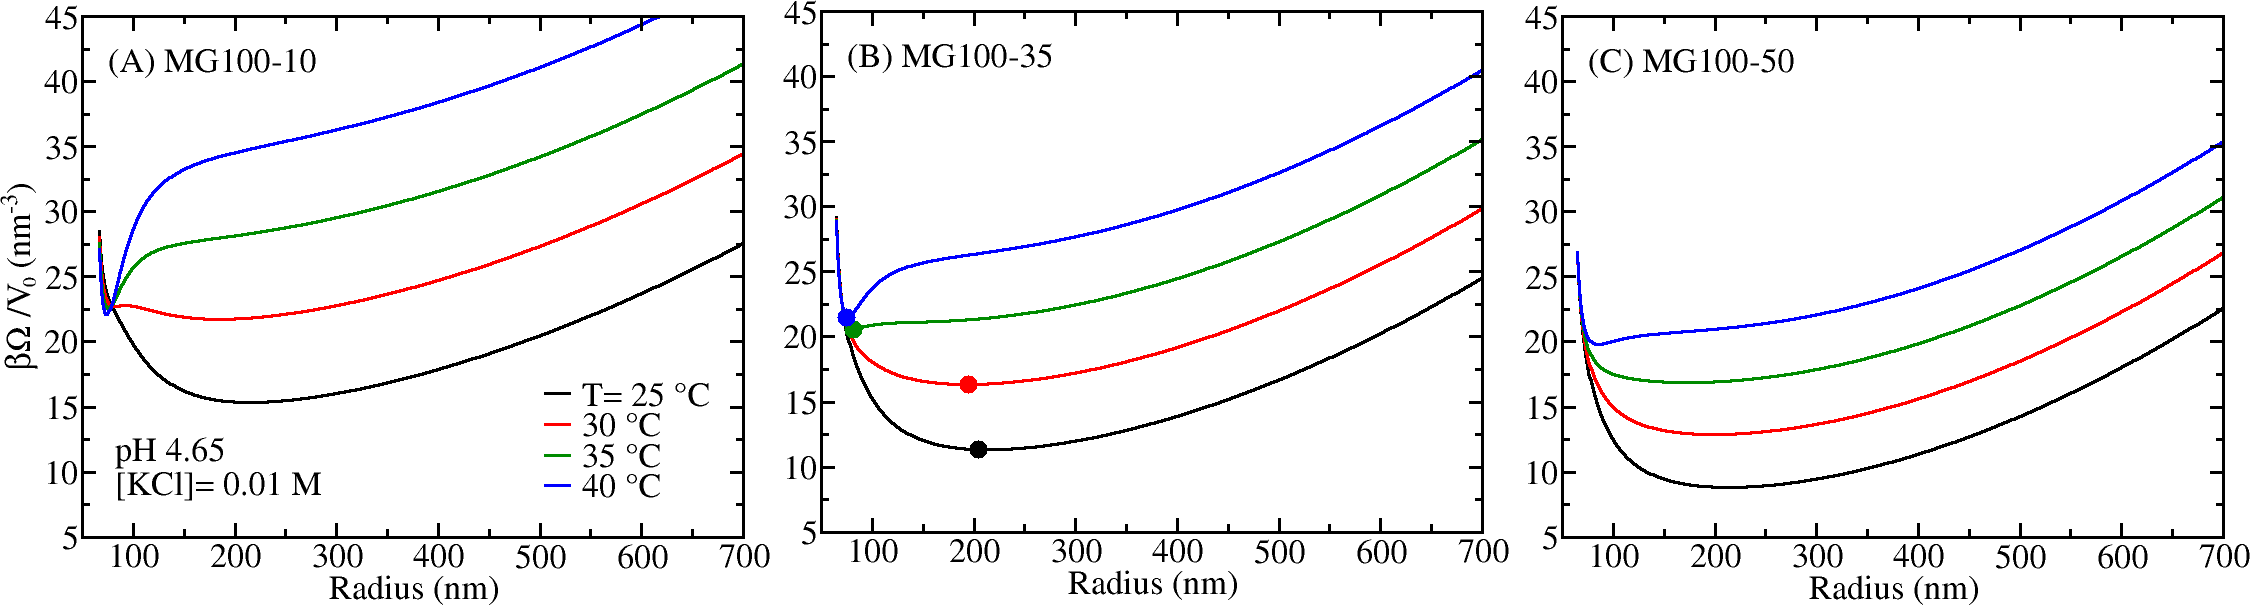
\includegraphics[width=1.\linewidth]{Figures/graph-gel/graph-min.png}
\caption{Thermodynamic potential as a function of the microgel radius at different temperatures, $pH~4.65$ and $cs=10^{-2}M$.
Each panel corresponds to a different MG100 microgel (chain length, $n_{ch}=100$) with $10\%$ (A), $35\%$ (B), and $50\%$ (C) MAA.
The plots present the thermodynamic potential in excess of the solution contribution, $\Omega=\Omega_{MG}-\Omega_s$, in some convenient units, where $V_0=\frac{4}{3}\pi R_0^3$ is the volume of the dry polymeric particle.
In panel B, a color circle marks the optimal radius for each temperature, which is the local/global minimum of the corresponding curve (see tabla \ref{table:optimal-R}).}
\label{fig:graph-min}
\end{figure*}


At this point, we can completely determine the free energy of the microgel phase for any given $R$.
The independent variables of a calculation are the temperature, the pH and salt concentration of the embedding solution.
The number of segments in the polymer network $N_{seg}$, the chain length $n_{ch}$, and the fraction of MAA segments, $x_{MAA}$, fully characterize the microgel.


We consider microgels with $N_{seg}=10^7$ segments and $n_{ch}=50$, $100$, and $200$, having either $x_{MAA}=0.1$, $0.35$ or $0.5$.
Our goal is to evaluate the effect of increasing or reducing the amount of acidic monomer with respect to poly(NIPAm-\emph{co}-MAA) microgels having $35\%$ MAA, which are typically synthesized in our lab \addcite[Giussi2015,Giussi2020].
These microgels are labeled MG$n_{ch}$-$p_{MAA}$, where $p_{MAA}$ is the percentage of MAA.
For example, MG100-10 is the microgel with  $n_{ch}=100$ and $x_{MAA}=0.1$.






To determine the size of the microgel for a given set of conditions, we resource to a graphical minimization procedure.
For each set of conditions (pH, salt, and $T$), we construct $\Omega(R)=\Omega_{MG}(R)-\Omega_{s}(R)$, and find $R_{opt}$, the optimal radius, such that the curve has a local (and global) minimum.
As an example, this procedure is illustrated in figura \ref{fig:graph-min} for MG100 microgels.
The results obtained from the graphical minimization of figura \ref{fig:graph-min} curves are summarized in tabla \ref{table:optimal-R}.



\begin{table}[!htb]
\centering
\small
  \begin{tabular}{|lccccc|}
   \hline %\multirow{2}{*}{MG100} & 
    %  \multicolumn{4}{c}{Opt. Radius (nm)(MG100)} \\
    	&&   Opt. Radius (nm)(MG100 & && \\
    	\hline
      & {25 $^\circ C$} & {30 $^\circ C$} & {35 $^\circ C$} & {40 $^\circ C$} & {dry, $R_0$} \\
      \hline
    10\% MAA & 215 &  184 &  75  &  74 & 65\\
    35\% MAA &  213 &  193 &  84 & 76 & 64\\
    50\% MAA &  213 & 199 &  172 & 85 & 63\\
    \hline
  \end{tabular}
 \caption{Graphical minimization of figura \ref{fig:graph-min} curves.
 This table summarizes the optimal radii of three MG100 microgels at different temperatures, $pH\,4.65$ and $cs=10^{-2}M$.}
\label{table:optimal-R} 
\end{table}


\subsection{Absorption}
%%%%%%%%%%%%%%%%%%%%%%%%%%%%%%%%%%%%%%%%%%%%%%%%%%%%%%%%%%%%%%%%%%%%%




To describe the absorption of an analyte to the microgel phase, 
the thermodynamic potential of eq. \ref{eq:free-energy} adds the following terms:
%
%
\begin{align}
\begin{aligned}
\beta&\frac{\Omega_{MG}(R)}{V}= \cdots\\&+ \rho_a\left(\ln\left(\rho_a v_w\right) -1 + \beta\mu^0_a\right) \\
& + \rho_a \sum_\tau n_\tau  \left[g_\tau(\ln g_\tau+ \beta\mu^0_{\tau})\right.\\
&\qquad\left.+(1-g_\tau)(\ln (1-g_\tau)+\beta\mu^0_{\tau H})\right] \\
& +  \left( \rho_a \sum_\tau n_\tau f_\tau q_\tau\right)\beta\psi_{MG}\\
& -\rho_a\beta\mu_a
 -\beta\mu_{H^+} \rho_a \sum_\tau n_\tau g_\tau
\end{aligned}
\label{eq:ads}
\end{align}
%
\noindent The first line (right-hand side) accounts for the translational degrees of freedom,
where $\rho_a$ is the number density of the analyte and $\mu_a^0$ its standard chemical potential.
The next two lines describe the acid-base equilibrium of titratable units of the analyte;
subscript $\tau$ runs over such molecular units having degree of protonation $g_\tau$ and volume $v_\tau$.
The analyte has $n_\tau$ of these segments;
$\mu^0_{\tau H}$ and $\mu^0_\tau$ are the standard chemical potential of the protonated and deprotonated species, respectively, which relate to the acid dissociation constant:
%
\begin{align}
K^0_{\tau}= e^{\beta\mu^0_{\tau H}-\beta\mu^0_{\tau}-\beta\mu^0_{H^+}}
\end{align}
%

The next line in eq. \ref{eq:ads} describes the analyte contribution to the electrostatic energy, where $f_\tau$ is the degree of charge of $\tau$ units, which is either equal to $g_\tau$ if $\tau$ is a basic group, or $(1-g_\tau)$ if the unit is acidic; $q_\tau$ is the charge of the ionized species.
The last two terms account for the chemical equilibrium between the microgel and the solution phase, where $\mu_a$ is the chemical potential of the analyte.



In addition, eq. \ref{eq:packing} must incorporate the total fraction of volume occupied by the analyte: $\rho_a \sum_\lambda n_\lambda v_\lambda$, where $\lambda$ runs over all types of segments that make the molecule, including titratable units $\{\tau\}\in\{\lambda\}$.
The presence of the analyte in the solution phase also represents additional contributions to the thermodynamic potential $\Omega_s$ of eq. \ref{eq:bulk}, which contain the same components as eq. \ref{eq:ads}. 


Optimization of $\Omega_{MG}$  leads to:
%
\begin{equation}
\frac{f_\tau}{1-f_\tau}=\left(\frac{K^0_\tau}{a_{H^+}}\right)^{\pm 1} e^{-\beta \psi_{MG} q_\tau}
\label{eq:f_ads}
\end{equation}
%
\noindent for the degree of charge of $\tau$ units, where the $\pm$ sign differentiates the case of an acid ($+$) from a basic ($-$) group.
For the analyte density we obtain:
%
\begin{align}
    \begin{aligned}
   \rho_a v_w =&\frac{ \exp{\left(\beta \mu_a - \beta \mu^0_a \right)}}{\prod_\tau \left(1-f_\tau\right)^{n_\tau}}\\
&\quad \cdot\exp{\left(-\beta \pi_{MG} \sum_\lambda n_\lambda v_\lambda \right)} 
    \end{aligned}\label{eq:rho_ads}
\end{align}
%
\noindent where this last equation requires a redefinition of $\mu_a$ and $\mu_a^0$.
Similar expressions to eq. \ref{eq:rho_ads} and eq. \ref{eq:f_ads} are derived for the solution phase.







\begin{figure}[!tb]
\centering
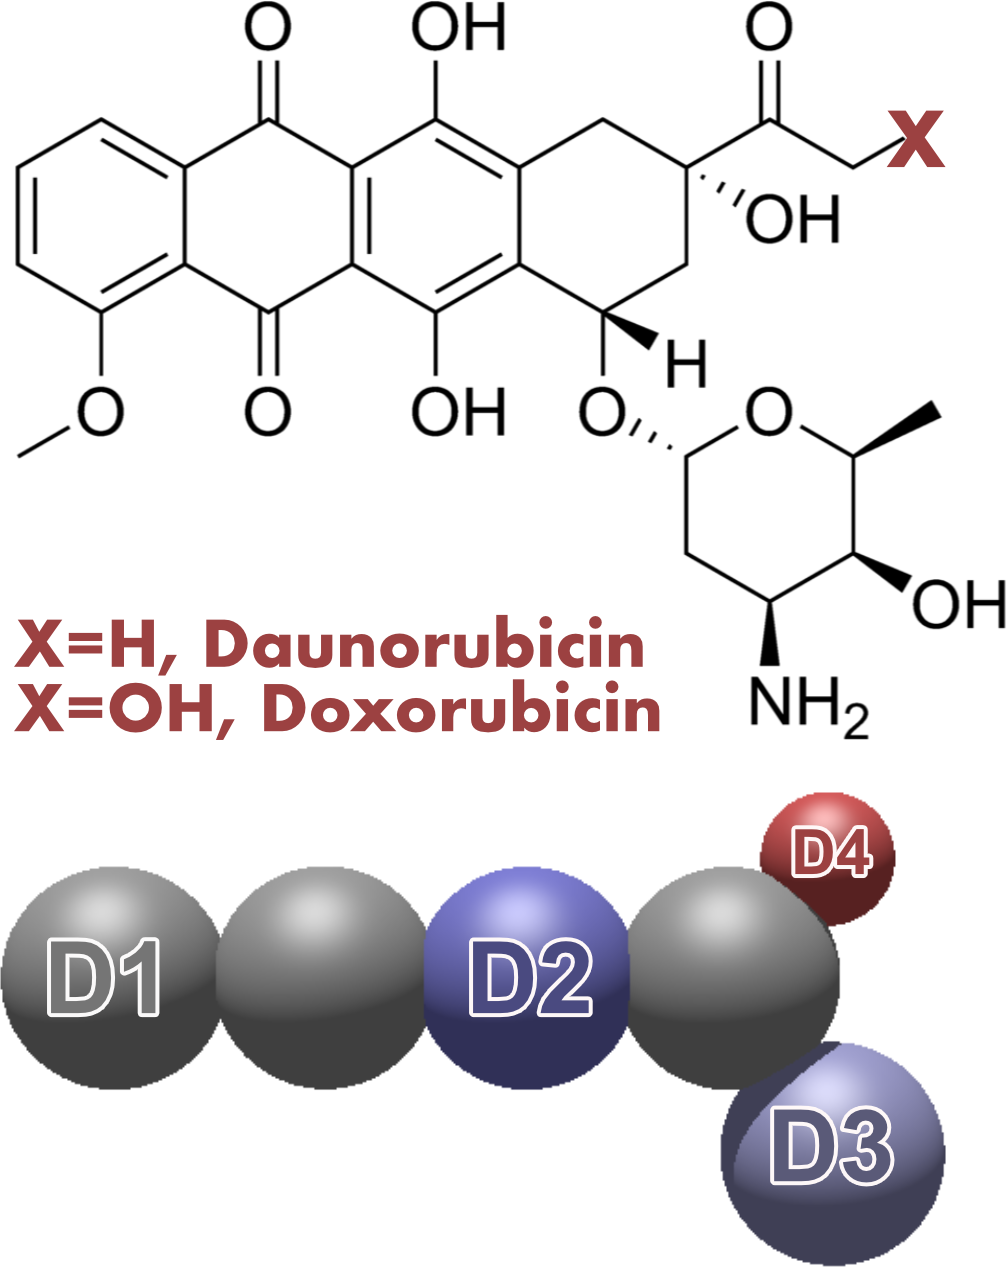
\includegraphics[width=0.35\linewidth]{Figures/graph-gel/dauno-doxo.png}
\caption{Chemical structure (top) and coarse grained model (bottom) applied to describe Daunorubicin and Doxorubicin.
The coarse grained segments $D1-D4$ are described in tabla \ref{table:drugs}.}
\label{fig:dauno-doxo}
\end{figure}



We will consider the absorption of the chemotherapeutic drugs Daunorubicin (Dauno) and Doxorubicin (Doxo) to the P(NIPAm-MAA) microgels under different conditions.
The molecular model applied to describe these analytes is illustrated in figura  \ref{fig:dauno-doxo} and the parametrization is presented in tabla \ref{table:drugs}.\addcite[PerezChavez2020]


\begin{table}
%\small
%\begin{tabular}{lcS[table-format=-1]S[table-format=0.3]}
\centering
\begin{tabular}{|lccc|}
    \hline
    {CG unit} & {$pKa$} & {$q$ ($e$)} & {$v$ ($\text{nm}^3$)} \\
      \hline
$D1$ & - & 0 & 0.085\\
$D2$ & 7.34 & -1$^\ast$ & 0.085\\
$D3$ & 9.46 & +1$^\ast$ & 0.085\\ 
$D4$ (Doxo) & 8.46 & -1$^\ast$ & 0.035\\
$D4$ (Dauno) & - & 0 & 0.035 \\
    \hline
  \end{tabular}
 \caption{Molecular properties of the different coarse grained units used to model Daunorubicin and Doxorubicin (see figura \ref{fig:dauno-doxo}).
\footnotesize ($^\ast$For the ionized unit.)}
\label{table:drugs} 
\end{table}




\section{Results and Discussion}
%%%%%%%%%%%%%%%%%%%%%%%%%%%%%%%%%%%%%%%%%%%%%%%%%%%%%%%%%%%%%%%%%%%%%



%%%%%%%%%%%%%%%%%%%%%%%%%%%%%%%%%%%%%%%%%%%%%%%%%%%%%%%%%%%%%%%%%%%%%
\subsection{Response to pH and Salt Concentration}\label{sec:pH_salt}
%%%%%%%%%%%%%%%%%%%%%%%%%%%%%%%%%%%%%%%%%%%%%%%%%%%%%%%%%%%%%%%%%%%%%


\begin{figure}[!ht]
\centering
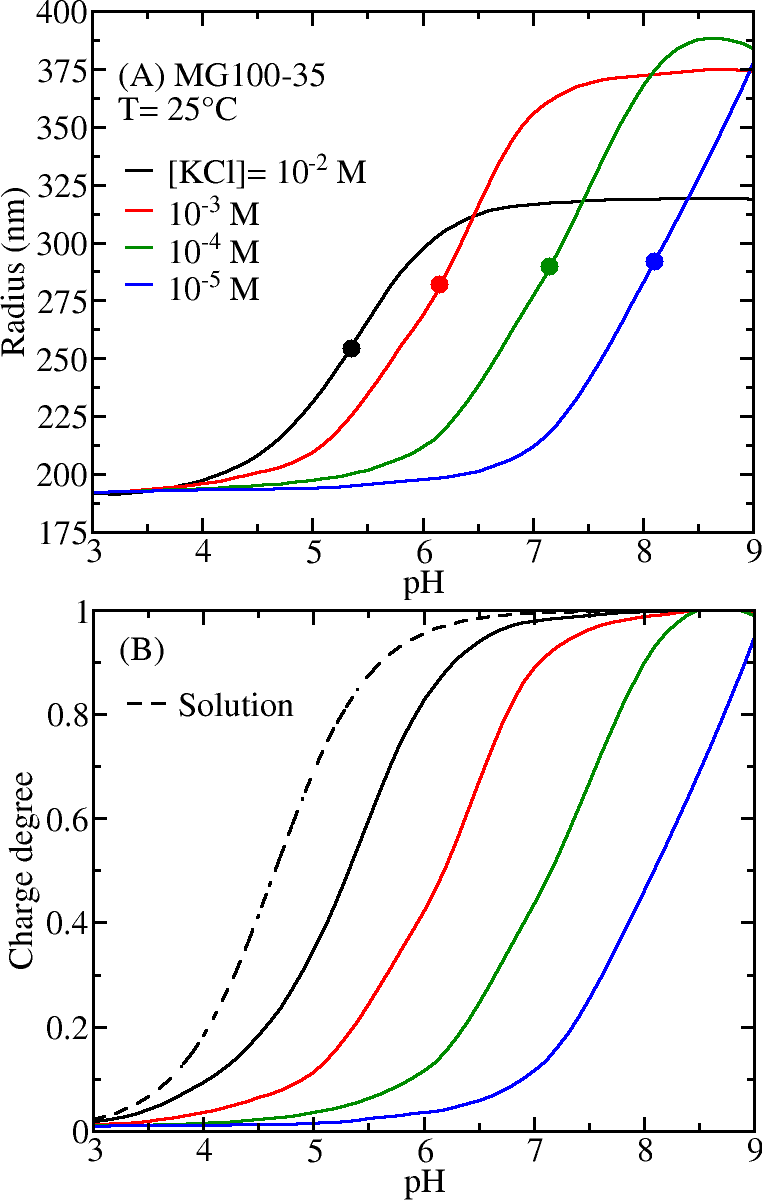
\includegraphics[width=0.5\linewidth]{Figures/graph-gel/R-pH.png}
\caption{Plot of microgel size (A) and degree of charge (B) as a function of pH for solutions having different salt concentrations and $T=25 ^\circ C$.
Polymer chains in the MG100-35 microgel are $n_{ch}=100$-long having $35\% $ MAA.
The dashed-line curve in panel B is the ideal dissociation of methacrylic acid ($pKa=4.65$).
Color circles on the curves of panel A mark the microgel apparent pKa.}
\label{fig:R-pH}
\end{figure}


In this section, we will describe the behavior of the microgels in response to changes in the composition of the embedding solution.
We concentrate on temperatures below that of PNIPAm LCST;
the effect of temperature will be evaluated in \ref{sec:temperature}.

Figura \ref{fig:R-pH}A shows the microgel size (radius, $R$) as a function of pH for different salt concentrations.
P(NIPAm-MAA) microgels swell with increasing pH.
As the pH is raised, an increasing number of MAA units deprotonate and become charged.
fihura \ref{fig:R-pH}B shows how the fraction of charged MAAs ($f$: degree of charge; see eq. \ref{eq:fcharge}) depends on the solution pH.
The microgel swelling observed in panel A as pH rises is the response to the growing intra-network repulsions that result from the increasing electric charge on the polymer seen in panel B.



The onset of the swelling transition displaces to higher pH values when lowering the salt concentration (salt, fig. \ref{fig:R-pH}A).
The proton dissociation curves of panel B present the same displacement to higher pHs, with respect to the ideal behavior of an isolated MAA monomer in dilute solution.
The apparent pKa of a microgel is the pH at which half of MAA segments are deprotonated;
it quantifies the microgel charging behavior, fig. \ref{fig:R-pH}B, but also the swelling transition as we see in panel A (see circles at $pH=pKa$).
The apparent pKa's of fig. \ref{fig:R-pH}B are displayed in tabla \ref{table:pKa_app}.


\begin{table}[!htb]
\small
  \begin{tabular}{|cc|}
    \hline
      [salt] (M)& App. pKa ($25 ^\circ C$)  \\
      \hline
    $10^{-5}$ & 8.10  \\
    $10^{-4}$ & 7.15 \\
    $10^{-3}$ & 6.15 \\
    $10^{-2}$ & 5.35 \\
    %\azul $10^{-1}$ & \azul 4.80 \\
    ideal (pKa) &  $4.65$  \\
    \hline
  \end{tabular}
 \caption{Apparent pKa's of fig. \ref{fig:R-pH} for a MG100-35 at $25 ^\circ C$.}
\label{table:pKa_app} 
\end{table}



A relatively high concentration of salt ions inside the microgel, results in the screening of the electrostatic repulsions between charged MAA segments;
effectively, these repulsive interactions become short range.
When the solution pH increases, MAA dissociation proceeds without a high energetic cost of electrostatic repulsions.
Under these conditions MAA deprotonation, induced by the chemical free energy (acid-base equilibrium), approaches the ideal or dilute solution behavior (compare the high-[salt] cases with the dashed-line curve in fig. \ref{fig:R-pH}B).



On the contrary, the screening effect weakens and intra-network electrostatic repulsions are effectively longer range for low salt concentration solutions.
Even if few distant charges appear on the network, they will interact with each other.
To reduce the energetic contribution of such electrostatic repulsions, MAA units are significantly less likely to be charged under low salt conditions;
the apparent pKa increases.
The price to pay instead is increasing the chemical free energy, whose contribution is minimized when the degree of protonation is ideal.


\begin{figure*}[!htb]
	\centering
	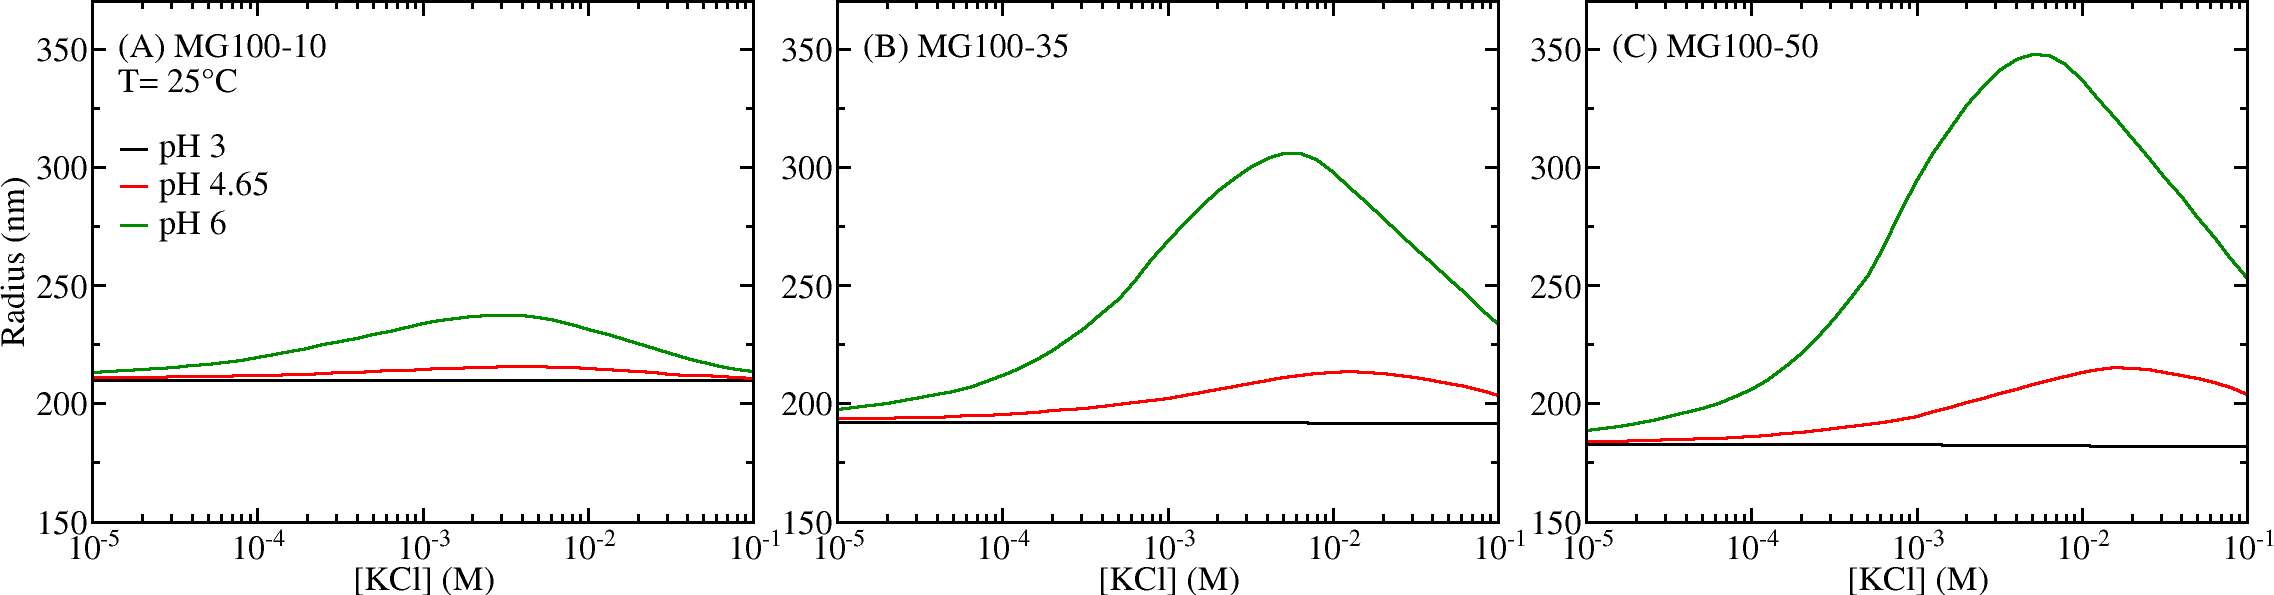
\includegraphics[width=1\linewidth]{Figures/graph-gel/R-cs.png}
	\caption{Plot of the microgel size as a function of the salt concentrations for different pH solutions and $T=25 ^\circ C$.
		The panels correspond to MG-100 microgels (chain length, $n_{ch}=100$) having MAA fractions: $10\%$ (A), $35\%$ (B) and $50\%$ (C).}
	\label{fig:R-cs}
\end{figure*}




Figura \ref{fig:R-cs} illustrates how the size of P(NIPAm-MAA) microgels depends on the salt concentration for different values of pH.
At relatively high salinity, these microgels deswell with increasing salt concentration, which is consistent with the dynamic light scattering (DLS) results of \addcite[citet:Wong2009]  for P(NIPAm-MAA) microgels and NaCl concentrations in the range $0.1-0.5 M$.

The curves of Figura \ref{fig:R-cs} display a re-entrant behavior, in which the size first increases and then decreases when raising the salt concentration.
This nonmonotonic response is more prominent when the polymer charge increases due to either a higher pH or MAA content (compare different panels of firgura \ref{fig:R-cs}).



Swelling-deswelling transitions with varying salt concentration have been reported for a variety of charge-regulating polymeric systems.
The thickness of layers of grafted weak polyacids is a nonmonotonic function of the solution salt concentration as predicted by scaling and self-consistent mean-field theory \addcite[Israels1994,Lyatskaya1995,Zhulina1995,Gong2007], which has been confirmed by experimental results \addcite[Wu2007].
Similarly, theoretical results predict that the size of star-branched weak polyelectrolytes displays a maximum as function of the solution salt concentration \addcite[Borisov1998,KleinWolterink2002]; 
the thickness of grafted films of crosslinked weak polyacids has also been predicted to show this re-entrant swelling behavior \addcite[Longo2014JCP].



A salt-driven deswelling to swelling transition has been predicted for strong polyelectrolyte nanogels \addcite[jha2012understanding];
this behavior, in the case of quenched polyelectrolytes, was attributed to excluded volume effects of absorbed ions at high salt concentrations.
More relevant to our study, a re-entrant swelling-to-collapse transition was theoretically predicted for pH- and thermoresponsive microgels \addcite[polotsky2013collapse].
\addcite[citet:polotsky2013collapse] explain that increasing salt concentration first promotes charge dissociation of the weak acid groups until saturation is achieved when the degree of dissociation reaches the ideal value. 
Beyond this point, increasing the salt concentration of the solution only enhances the screening of the electrostatic repulsions, and thus the microgel deswells.
Experimentally, the nonmonotonic swelling of poly(NIPAm-\emph{co}-AA) (P(NIPAm-AA)) microgels as a function of NaCl concentration was reported by \addcite[citet:CaprilesGonzalez2008] using DLS.
